%%%%%%%%%%%%%%%%%%%%%%%%%%%%%%%%%%%%%%%%%%%%%%%%%%%%%%%%%%%%%%%%%%%%%%%%
\chapter{Introduction}
\label{chapter:introduction}
%%%%%%%%%%%%%%%%%%%%%%%%%%%%%%%%%%%%%%%%%%%%%%%%%%%%%%%%%%%%%%%%%%%%%%%%
\localtableofcontents

\section{Context}

Neural networks are now present all around us and in all areas.
Without knowing it, an average person uses them every day; automatic translators, chatbots, voice assistants, recommendations, etc.
The applications are very diverse and can have a profound impact on entire sectors (transport, health care, etc.).
If the use of neural networks is so important, it is because they are so effective in \emph{learning} any type of task with results that are close to perfection, surpassing man on many points.

However, although widely in use, Neural Networks are not perfect, a lot of open questions remain and many problems have emerged.
This thesis attempts to highlight and answer some of the problems that Neural Networks face.

\section{Introduction to Neural Networks}

Neural Networks find their roots, in 1958, in the works of Frank Rosenblatt \cite{rosenblatt1958perceptron} where for the first time, the Perceptron, an electronic device inspired by the human brain, showed ability to \emph{learn} from multiple examples.
In essence, the Perceptron is an algorithm for learning a binary classifier, this classifier can be analytically described as a composition of a linear function $\phi$ and the Heaviside step function $\rho$ as follows:
\begin{equation}
  f(\xvec) = \rho \circ \phi(\xvec) = \left\{ 
    \begin{aligned}
      &1 \quad \text{if} \quad \phi(\xvec) > 0  \\
      &0 \quad \text{otherwise}
    \end{aligned}
    \right. .
\end{equation}
where $\phi(\xvec) = \wvec^\top \xvec$ is a linear function and the values of the vector $\wvec$ are the learned parameters. 
However, a few years after its introduction, \citet{minsky1969perceptrons} demonstrated important limitations of the Perceptron.
Indeed, although theoretically capable of classifying any linear separable problem, it is not able to correctly classify simple non-linear functions (see Figure~\ref{figure:xor_function}).
\begin{figure}[htb]
  \centering
  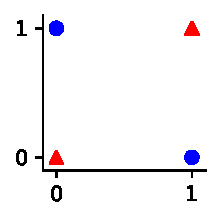
\includegraphics{figures/chapter1/xor_function.pdf}
  \caption{Graphical representation of the XOR function. This function cannot be separated by a linear classifier.}
  \label{figure:xor_function}
\end{figure}
To circumvent these limitations, \citet{minsky1969perceptrons} considered that an \emph{other layer of logic} could be added to the function allowing the classification to be done on another representation (see Figure~\ref{figure:multi_layer_perceptron}).
Let $\phi_1$ and $\phi_2$ be two linear functions, we could define a \emph{Multi-Layer Perceptron} as follows:
\begin{equation}
  f(\xvec) = \rho \circ \phi_2 \circ \rho \circ \phi_1( \xvec )
\end{equation}

\begin{figure}[ht]
  \centering
  \begin{subfigure}[t]{0.30\textwidth}
    \centering
    \begin{tabular}{c|c}
      \multicolumn{2}{c}{$\xvec$} \\
      \midrule
      0 & 0 \\
      0 & 1 \\
      1 & 0 \\
      1 & 1
    \end{tabular} 
    \caption*{Input representation}
  \end{subfigure}
  \begin{subfigure}[t]{0.03\textwidth}
    $\rightarrow$
  \end{subfigure}
  \begin{subfigure}[t]{0.30\textwidth}
    \centering
    \begin{tabular}{C{0.5cm} | C{0.5cm}}
      \multicolumn{2}{c}{$\rho \circ \phi_1(\xvec)$} \\
      \midrule
      0 & 0 \\
      0 & 1 \\
      1 & 0 \\
      0 & 0
    \end{tabular}
    \caption*{Intermediate representation}
  \end{subfigure}
  \begin{subfigure}[t]{0.03\textwidth}
    $\rightarrow$
  \end{subfigure}
  \begin{subfigure}[t]{0.30\textwidth}
    \centering
    \begin{tabular}{c}
      $f(\xvec)$ \\
      \midrule
      0 \\
      1 \\
      1 \\
      0
    \end{tabular}
    \caption*{Final representation}
  \end{subfigure}
  \caption{Classification of the XOR function with a Multi-Layer Perceptron}
  \label{figure:multi_layer_perceptron}
\end{figure}


One of the first \emph{Multi-Layer Perceptron}, or now more commonly known as \emph{Deep Neural Network}, was introduced by~\citeauthor{ivakhnenko1967cybernetics} in~\citeyear{ivakhnenko1967cybernetics}.
More precisely, a Neural Neural can be analytically described as a composition of linear function interlaced with non-linear function (also called activation function):
\begin{equation}
  f_\Wmat(\xvec) = \phi_{\Wmat_L} \circ \rho \circ \phi_{\Wmat_{L-1}} \circ \cdots \circ \phi_{\Wmat_2} \circ \rho \circ \phi_{\Wmat_1}(\xvec)
  \label{equation:neural_network}
\end{equation}
where the function $\phi_{\Wmat_i}$ is a linear function parameterized by $\Wmat_i$, $\rho$ is a non-linear function (also called activation function), $\Wmat = \{\Wmat_1, \dots, \Wmat_L \}$ and $L$ correspond to the \emph{depth} of the network (\ie the number of layers).

In recent years, Deep Neural Networks have achieved state-of-the-art performances in a variety of domains such as image recognition~\cite{lecun1998gradient,krizhevsky2012imagenet,He_2016_CVPR,tan2019efficientnet}, image detection~\cite{redmon2016you}, natural language processing~\cite{radford2018Language}, speech recognition~\citet{hinton2012deep}, etc. 
In order for Deep Neural Networks to achieve such performance, specific architectures have been devised for each application.
More precisely, each of these architectures relies on specific \emph{structured linear transformations}.


\section{Introducing Structure into Deep Neural Networks}

A neural network is a function $f:\Rbb^n \rightarrow \Rbb^m$ composed of at least two linear functions (layers) and one non-linear function (activation function).
The input space $n$ is usually large and the output space $m$ corresponds to the number of classes the network has to classify; therefore, we have $m \ll n$.
We can write two layers neural network as follows:
\begin{equation}
  f(\xvec) = \Wmat_2 \rho(\Wmat_1 \xvec)
  \label{equation:two_layer_neural_network}
\end{equation}
where $\Wmat_1 \in \Rbb^{n \times n}$, $\Wmat_2 \in \Rbb^{m \times n}$ are dense matrices.
This architecture is called \emph{Fully Connected Neural Network} because all the neurons from the first activation are connected to all the neurons from the second activation.
This type of network can have a large number of parameters, for example, with the MNIST dataset~\cite{lecun1998gradient} which consists of $28 \times 28$ images of hand-written digits from 0 to 9, the network from equation~\ref{equation:two_layer_neural_network} will have more than $6 \times 10^5$ parameters.



Training such a large network has a number of significant drawbacks: they are hard to train, subject to overfitting and are computationally expensive.
% To overcome these drawbacks, researchers have devised neural networks with specific linear operation which have considerably less parameters.
To overcome these drawbacks, researchers have devised neural networks with structure linear operations in order to reduce the number or parameters needed. 


\begin{figure}[ht]
   \centering
   \begin{subfigure}[t]{0.24\textwidth}
       \centering
       \begin{equation*}
	  \leftmatrix
	    a &   &   &   \\
	      & b &   &   \\
	      &   & c &   \\
	      &   &   & d
	  \rightmatrix
       \end{equation*}
       \caption*{diagonal}
   \end{subfigure}
   \hfill
   \begin{subfigure}[t]{0.24\textwidth}
       \centering
       \begin{equation*}
	  \leftmatrix
	    a & b & c & d \\
	    e & a & b & c \\
	    f & e & a & b \\
	    d & f & e & a
	  \rightmatrix
       \end{equation*}
       \caption*{Toeplitz}
   \end{subfigure}
   \hfill
   \begin{subfigure}[t]{0.24\textwidth}
       \centering
       \begin{equation*}
	  \leftmatrix
	    ae & af & ag & ah \\
	    be & bf & bg & bh \\
	    ce & cf & cg & ch \\
	    de & df & dg & dh
	  \rightmatrix
       \end{equation*}
       \caption*{Low Rank}
   \end{subfigure}
   \hfill
   \begin{subfigure}[t]{0.24\textwidth}
       \centering
       \begin{equation*}
	  \leftmatrix
	    a & a^2 & a^3 & a^4 \\
	    b & b^2 & b^3 & b^4 \\
	    c & c^2 & c^3 & c^4 \\
	    d & d^2 & d^3 & d^4
	  \rightmatrix
       \end{equation*}
       \caption*{Vandermonde}
   \end{subfigure}
  \caption{Examples of structured matrices.}
  \label{figure:example_structure_matrices}
\end{figure}


A $n \times n$ structure matrix can be represented with less than $n^2$ parameters, Figure~\ref{figure:example_structure_matrices} shows an example of structured matrices.
In addition to offering a more compact representation, the structure of certain matrices can be leveraged to obtain better algorithms for matrix-vector product leading in memory and computationally operations. 

Important questions remain, which structure is better suited for neural networks ? Does the reduction of parameters reduce the performance of the network ? Which properties can we leverage from these structures to improve the training and performance of neural networks ? 


% \subsection{Example of Structured Network: Convolutional Neural Network}


\begin{figure}[ht]
  \centering
  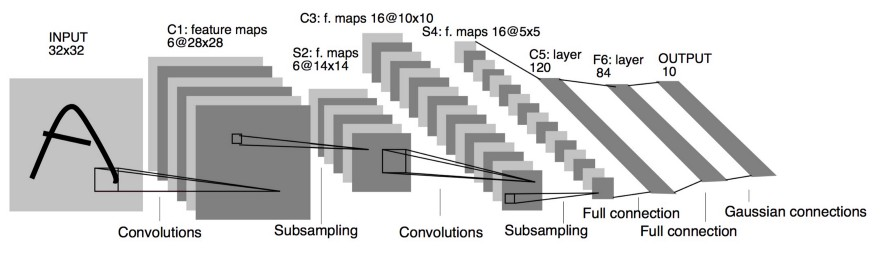
\includegraphics[scale=0.4]{figures/chapter1/lenet.jpg}
  \caption{Graphical representation of the LeNet architecture proposed by \citet{lecun1998gradient}}
  \label{figure:lenet_network}
\end{figure}

A perfect example of such efficient linear operation is the discrete convolution which consists of a kernel sliding over the image and acting as a filter.
Let $\avec$ and $\bvec$ be two complex-valued vectors indexed by the set $M = \{-m, -m+1, \dots, m-1, m\}$, the discrete convolution between the signals $\avec$ and $\bvec$ is given by: 
\begin{equation}
  (\avec \ast \bvec) \left[ n \right] \triangleq \sum_{m \in M} \avec\left[m\right] \cdot \bvec\left[n - m\right]
\end{equation}
The convolution operation has translation invariance characteristics \cite{zhang1990parallel} which is perfectly suited for image classification (objects can be at different positions in images).  
\citet{lecun1998gradient} was one of the first to successfully train a \emph{convolutional neural network} (CNN), achieving state-of-the-art performance on the MNIST dataset.
Convolution neural networks achieve such a great result for two main reasons:
first, CNNs are similar to the connectivity pattern of neurons in the visual cortex of the human brain. 
Secondly, CNNs are very efficient due to the sharing of parameters. 
While a classical linear operation with dense matrix has $n \times n$ parameters, a convolution only has $k \times k$ parameters where $k$ is the kernel size and is usually small (\eg 3 or 5 for classical convolution layers use in neural networks).
This weight sharing makes the network very small with respect to the Fully Connected neural network. The LeNet architecture (see Figure~\ref{figure:lenet_network}) has only $6 \times 10^4$ parameters.  

% From a Linear Algebra perspective, convolution can be expressed as a product between a matrix and the signal where the matrix is sparse with repetitive values. 

\section{Main contributions of the Thesis}

The contributions of this Thesis are based on structured matrices from the Toeplitz family.
More specifically, in Chapter~\ref{chapter:diagonal_circulant_neural_network}, we use circulant matrices, which are a particular case of Toeplitz matrices, to devise a new compact architecture replacing Fully Connected Neural Networks.
In Chapter~\ref{chapter:lipschitz_bound}, we leverage the structure of convolutional layers to devise a new regularization scheme for neural networks. 


In Chapter~\ref{chapter:diagonal_circulant_neural_network}, we study deep diagonal circulant neural networks, which are deep neural networks in which weight matrices are the product of diagonal and circulant ones.
Besides making a theoretical analysis of their expressivity, we introduce principled techniques for training these models: we devise an initialization scheme and propose a smart use of non-linearity functions in order to train deep diagonal circulant networks. 
Furthermore, we show that these networks outperform recently introduced deep networks with other types of structured layers.
We conduct a thorough experimental study to compare the performance of deep diagonal circulant networks with state-of-the-art models based on structured matrices and with dense models.
We show that our models achieve better accuracy than other structured approaches while requiring 2x fewer weights than the next best approach.
Finally, we train compact and accurate deep diagonal circulant networks on a real world video classification dataset with over 3.8 million training examples. 

Finally, in Chapter~\ref{chapter:lipschitz_bound}, we tackle the problem of Lipschitz regularization of Convolutional Neural Networks.
Lipschitz regularity is now established as a key property of modern deep learning with implications in training stability, generalization, robustness against adversarial examples, etc.
However, computing the exact value of the Lipschitz constant of a neural network is known to be NP-hard.
Recent attempts from the literature introduce upper bounds to approximate this constant that are either efficient but loose or accurate but computationally expensive.
In this work, by leveraging the theory of Toeplitz matrices, we introduce a new upper bound for convolutional layers that is both tight and easy to compute.
Based on this result we devise an algorithm to train Lipschitz regularized Convolutional Neural Networks.


